\documentclass{beamer}
\usepackage[utf8]{inputenc}
\usepackage{url}
\mode<presentation>
{
  \usetheme{Warsaw}       % or try default, Darmstadt, Warsaw, ...
  \usecolortheme{default} % or try albatross, beaver, crane, ...
  \usefonttheme{serif}    % or try default, structurebold, ...
  \setbeamertemplate{navigation symbols}{}
  \setbeamertemplate{caption}[numbered]
} 

% \usetheme{Marburg}
% \usecolortheme{orchid}

\newcommand{\QQ}{\mathbb{Q}}
\newcommand{\CC}{\mathbb{C}}

\title[Uniformization Theorem and Children's Drawings]{Riemann Surfaces through the Uniformization Theorem and Children's Drawings}
\author{Drimik Roy and Zach Halberstam}
\institute{University of Michigan}
\date{June 12, 2019}

\begin{document}
\begin{frame}
    \titlepage
\end{frame}
%Emphasize compatibility criterion
\begin{frame}{Riemann Surfaces}
\begin{definition}[Riemann Surface]
    A Riemann Surface is a 1-dimensional complex manifold; that is, a space that "looks like" the complex plane near every point.
\end{definition}
\begin{examples}
Riemann Sphere, $\CC$ 
\end{examples}
\begin{figure}
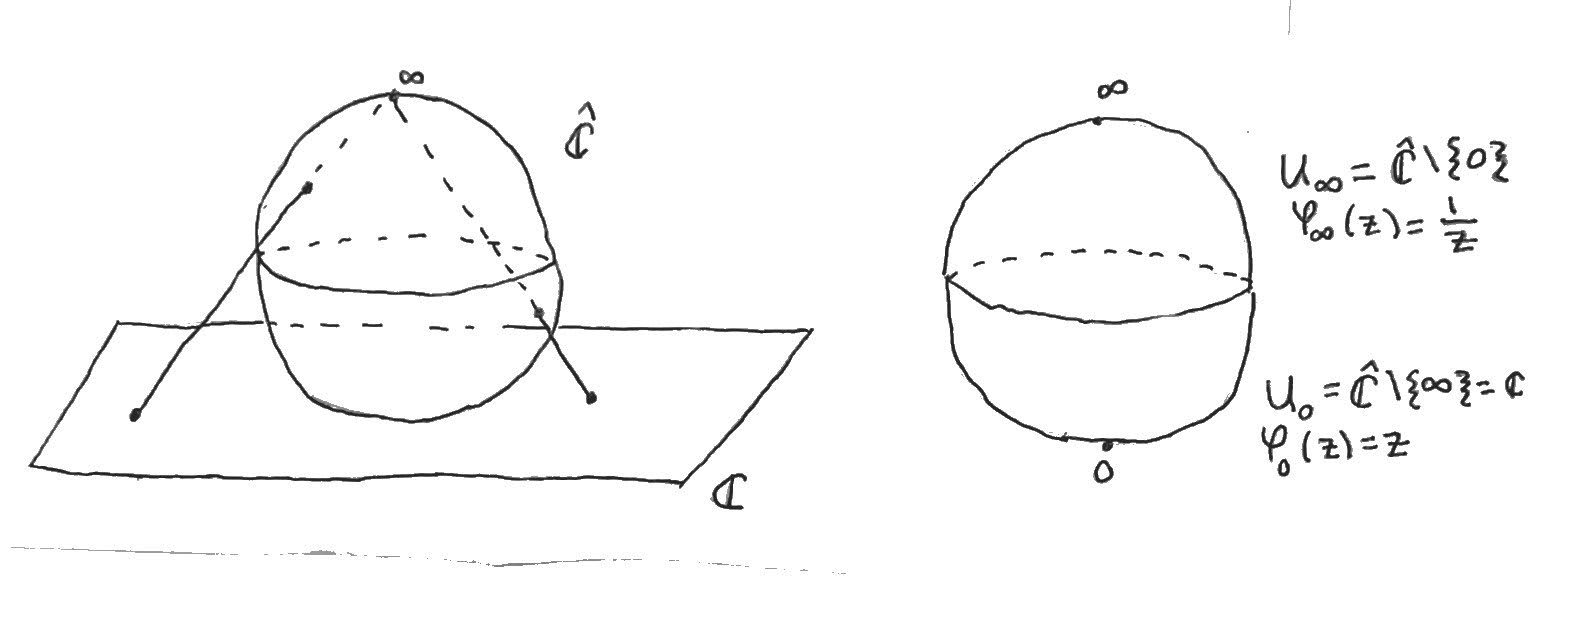
\includegraphics[scale=0.15]{images_talk/riemannsphere.jpeg}
\caption{Stereographic projection and an atlas for the Riemann Sphere}
\end{figure}

\end{frame}

\section{}
%Make sure to mention that the fundamental group of a path connected topological space does not depend on the base point, that S does not change as y changes, that is, that all points in Y have the same number of preimages
\begin{frame}{Covering Theory}
\begin{definition}[Covering]
For path connected spaces $X$, $Y$, and a continuous mapping $p:X\to Y$, $p$ is a \textit{covering} of $Y$ by $X$ if for all $y\in Y$, there exists a neighborhood $V$ of $y$ such that $p^{-1}(V)$ is of the form $\bigsqcup_{\alpha\in A} U_\alpha$, where each $U_\alpha$ is homeomorphic to $V.$  
\end{definition}
\begin{definition}[Fundamental Group]
For a pointed topological space $(X, x_0)$, the \textit{fundamental group} $\pi_1(X, x_0)$ is the set of homotopy classes of paths in $X$ starting and ending at $x_0$. The operation on the fundamental group is loop concatenation. 
\end{definition}
\begin{theorem}[The Path Lifting Property]
Let $p:X\to Y$ be a covering, let $\gamma: [0, 1]\to Y$ be a path, and let $p(x_0)=\gamma(0).$ Then, there is a unique path $\tilde{\gamma}: [0, 1]\to X$ such that $p(\tilde{\gamma})=\gamma$ and $\tilde{\gamma}(0)=x_0.$
\end{theorem}


    
\end{frame}
\begin{frame}{Universal Covers}
\begin{definitions}[Simply connected, Universal Cover]
A space $X$ is \textit{simply connected} if every loop in $X$ is contractible to a single point. A simply connected cover is called a \textit{universal cover.}
\end{definitions}
\begin{definition}[Galois Covering]
A covering $p:X\to Y$ is Galois if, if a loop in $Y$ lifts to a loop in $X$, it can never lift to a path in $X$ which is not a loop.
\end{definition}
\begin{block}{Fundamental Theorem of Galois Theory for Covering Spaces}
    If $X, Y$ are path connected and $p:X\to Y$ is a Galois covering, then:
    \begin{itemize}
        \item $p_*(\pi_1(X))$ is normal in $\pi_1(Y)$.
        \item The \textit{Deck group} $D(p),$ the group of automorphisms $d:X\to X$ such that $p\circ d=p$, is isomorphic to $\pi_1(Y)/p_*(\pi_1(X))$.
    \end{itemize}
\end{block}
\end{frame}

\begin{frame}{The Uniformization Theorem}
\begin{theorem}[The Uniformization Theorem]
   Up to biholomorphism, there are just three simply connected Riemann surfaces: the complex plane $\mathbb{C}$, the Riemann sphere $\hat{\mathbb{C}}$, and the upper half-plane $\mathbb{H}$.
\end{theorem}
\begin{block}{Corollary}
Every connected Riemann surface can be expressed as the quotient of $\hat{\mathbb{C}},$ $\mathbb{C},$ or $\mathbb{H}$ by a discrete group of automorphisms.
\end{block}
\begin{block}{Big Idea}
    We can construct Riemann surfaces as quotients of universal covers.
\end{block}
\end{frame}
\begin{frame}{Implications of Uniformization}

\begin{theorem}[Automorphisms of the universal covers]
\begin{itemize}
    \item The automorphisms of $\hat{\mathbb{C}}$ are $\text{PGL}(2, \mathbb{C}),$ i.e. of the form $f(z)=\frac{az+b}{cz+d}$ where $ad-bc\ne 0$ and $a, b, c, d\in \mathbb{C}.$
    \item The automorphisms of $\mathbb{H}$ are $\text{PSL}(2, \mathbb{R}),$ i.e. of the form $f(z)=\frac{az+b}{cz+d}$ where $ad-bc=1$ and $a, b, c, d\in \mathbb{R}.$
    \item The automorphisms of $\mathbb{C}$ are of the form $f(z)=az+b$ where $a, b\in \mathbb{C}$ and $a\ne 0.$
\end{itemize}
\end{theorem}
\begin{block}{Construction}
Every Riemann surface can be given a complex structure from the structure of its universal cover by taking the quotient of a discrete subgroup of automorphisms.
\end{block}
\end{frame}
\begin{frame}{Implications of Uniformization}

\begin{theorem}[\textbf{Isometries} of the universal covers]
\begin{itemize}
    \item The \textbf{isometries} of $\hat{\mathbb{C}}$ are $\text{P\textbf{S}L}(2, \mathbb{C}),$ i.e. of the form $f(z)=\frac{az+b}{cz+d}$ where $ad-bc\textbf{=1}.$ and $a, b, c, d\in \mathbb{C}.$
    \item The \textbf{isometries} of $\mathbb{H}$ are $\text{PSL}(2, \mathbb{R}),$ i.e. of the form $f(z)=\frac{az+b}{cz+d}$ where $ad-bc=1$ and $a, b, c, d\in \mathbb{R}.$
    \item The \textbf{isometries} of $\mathbb{C}$ are of the form $f(z)=az+b$ where $a, b\in \mathbb{C}$ and $|a|\textbf{=1}.$
\end{itemize}
\end{theorem}
\begin{block}{Construction}
Every Riemann surface can be given a \textbf{geometry} from the structure of its universal cover by taking the quotient of a discrete subgroup of \textbf{isometries}.
\end{block}
\end{frame}

\begin{frame}{Example}
\begin{figure}
    \centering
    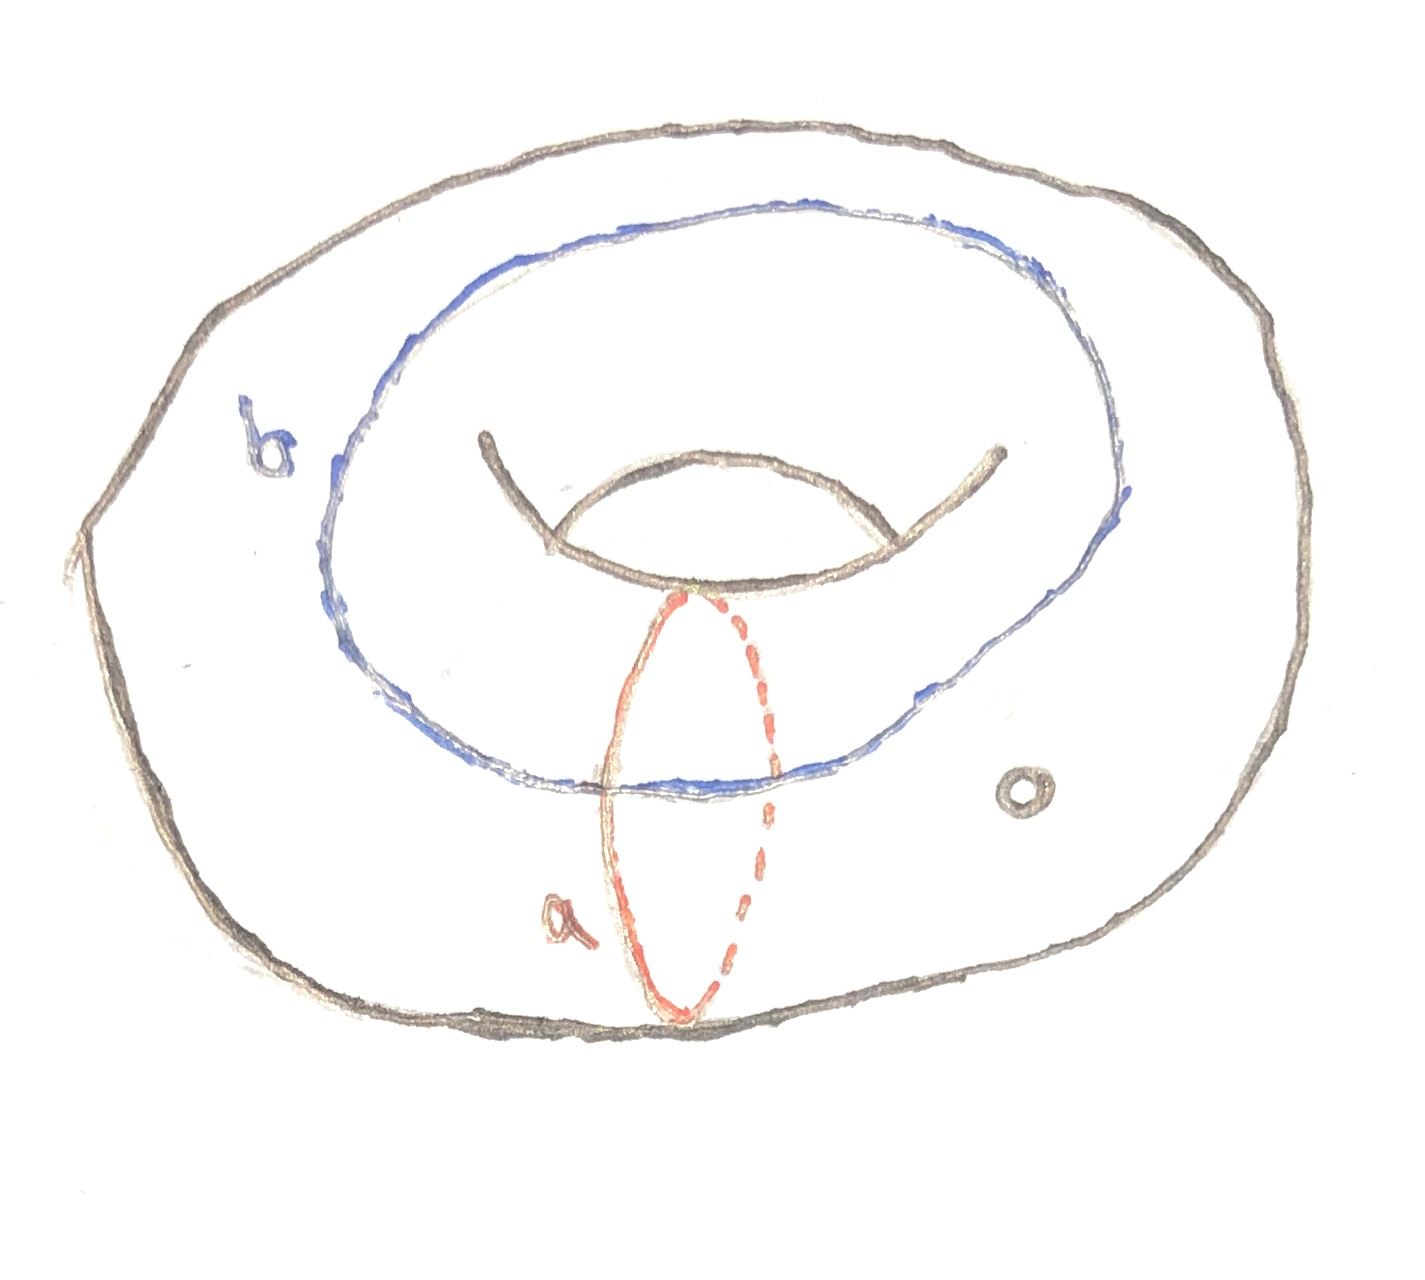
\includegraphics[width=0.5\textwidth]{images_talk/once-puncturedtorus.jpg}%
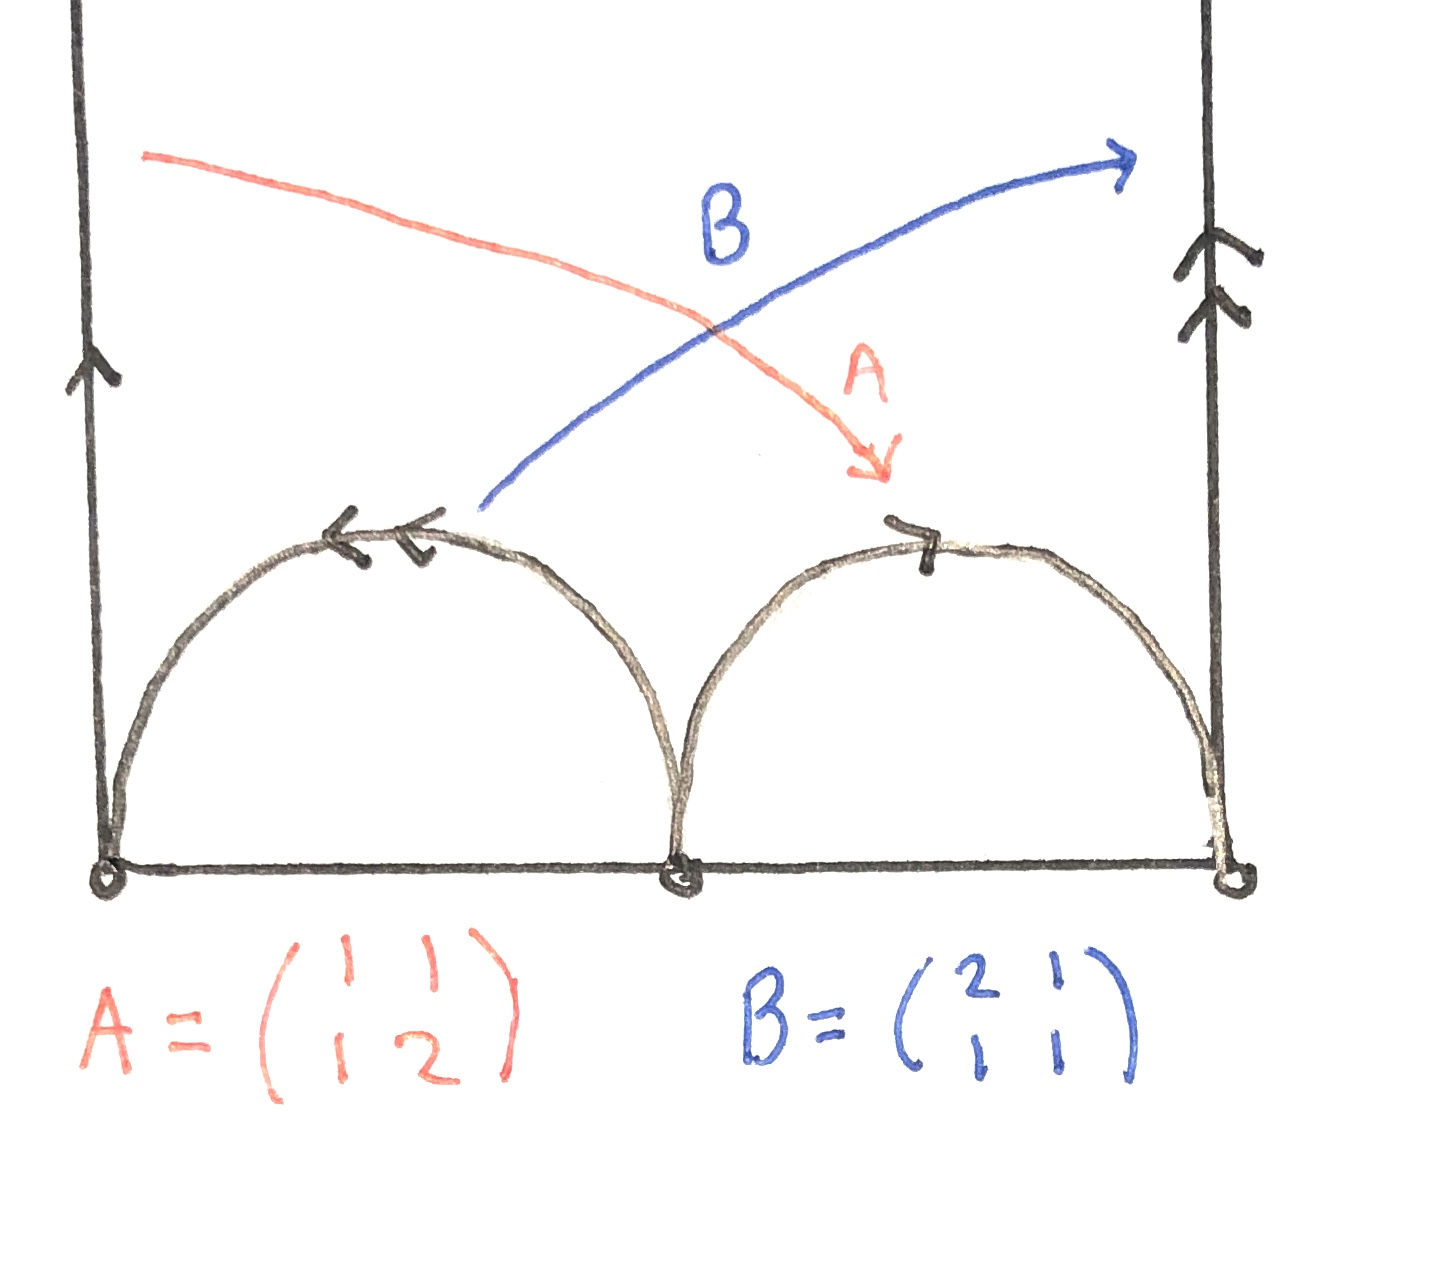
\includegraphics[width=0.5\textwidth]{images_talk/upper-half-planedecktransf.jpg}
    \caption{Once-punctured torus, and the upper-half plane with some automorphisms pictured}
    \label{fig:torusupperhalfplane}
\end{figure}
\end{frame}


%DDDDDRRRRRRRIIIIIMMMMMMIIIIIIIKKKKKK

% 1 MIN
% keywords: uniformization theorem
% Recap of key points from Zach
    % Uniformization tell us we can shift our problems to that of the universal cover and project them down
    % the fact that there are only 3 possible choices for complex analytic structures all of which we are familiar with gives us another tool to work with
    
    % construct RS by using the facts that fgrp should be isomorphic to the deck group defined for a covering map and just quotient the universal cover by discrete subgroup of automorphisms
% \begin{frame}{Ok.. so what of Uniformization?}
%     \begin{itemize}
%         \item Makes life easy
%         \begin{figure}
%         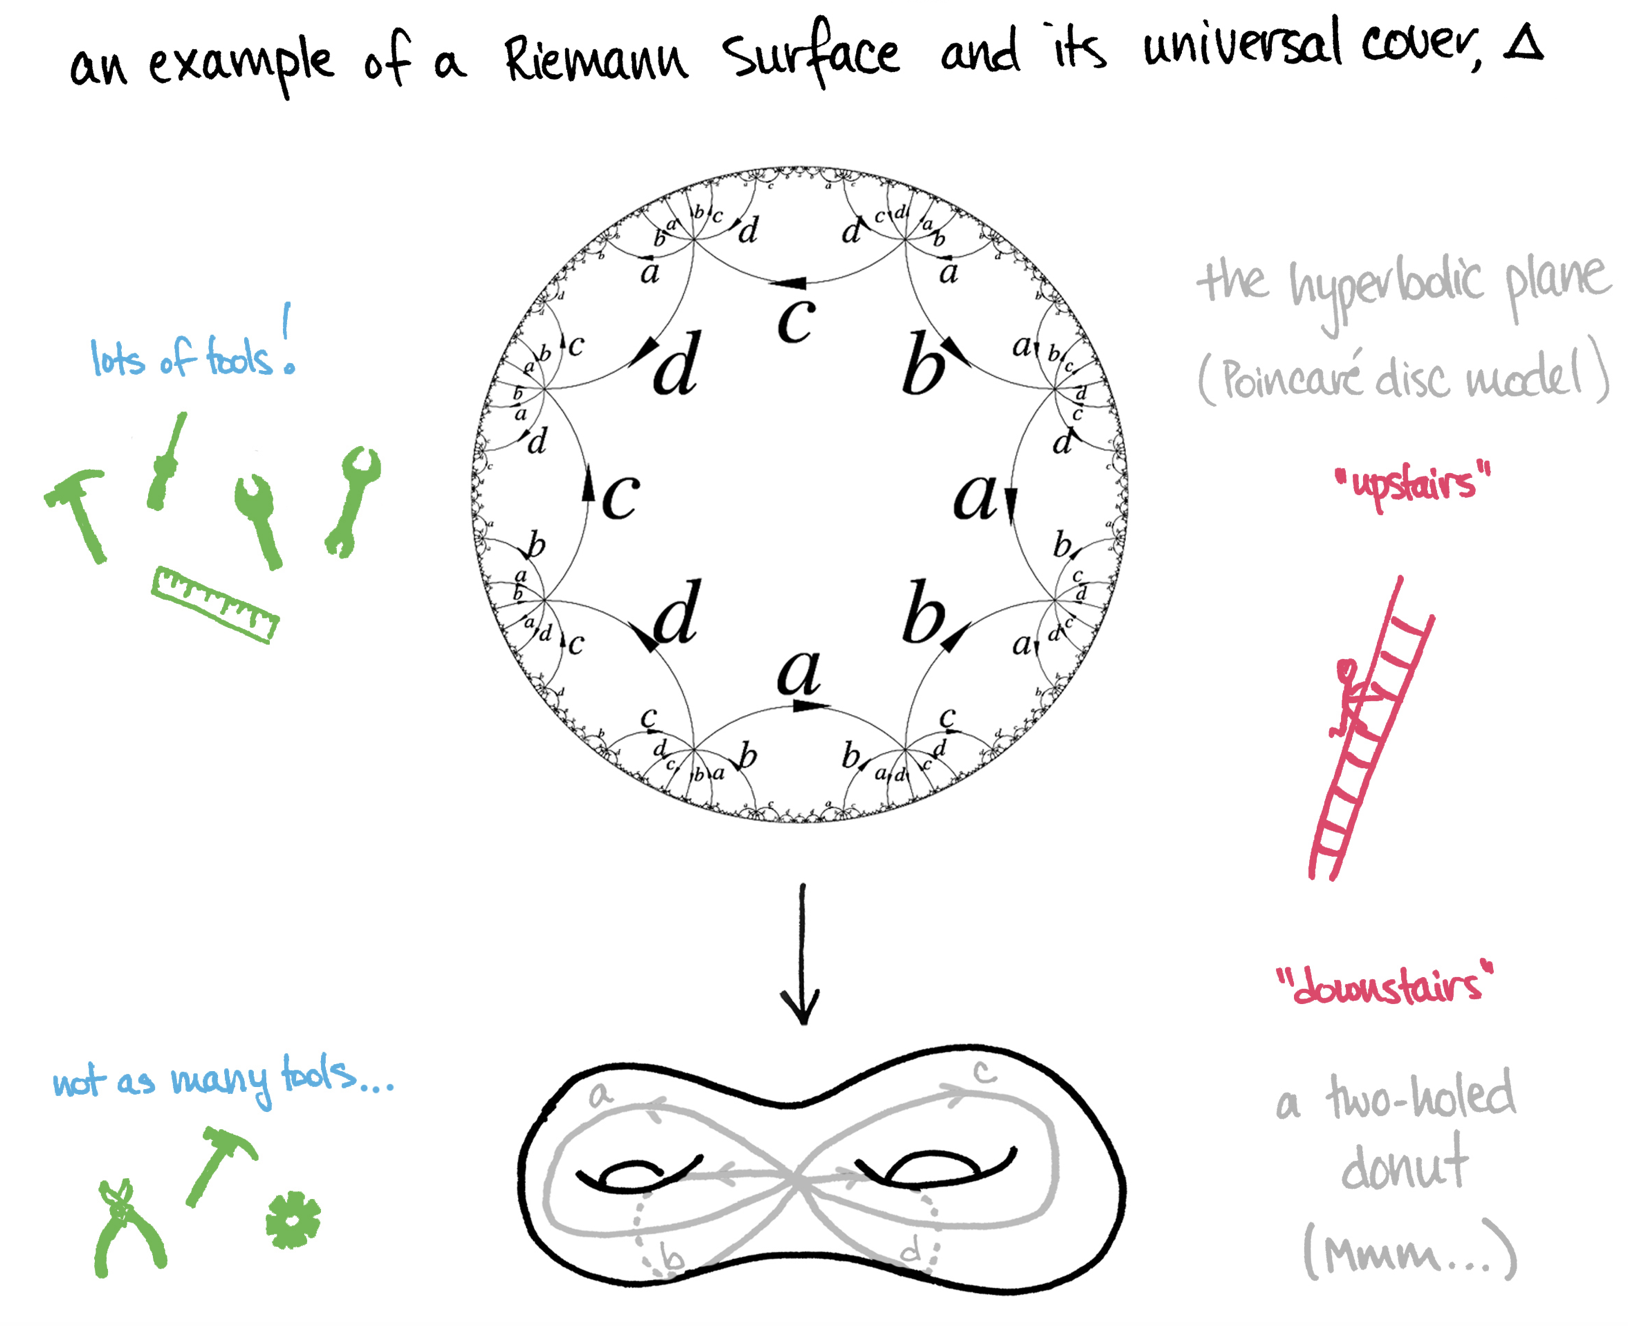
\includegraphics[scale=0.2]{images_talk/RS_uni_cover.png}
%         \caption{\small{Crisis averted \footnotemark}}
%         \end{figure}
%     \end{itemize}
%     \footnotetext[1]{\tiny \url{https://www.math3ma.com/blog/three-important-riemann-surfaces}}
% \end{frame}

\begin{frame}{}
    Theory of \emph{Dessin d'enfants} extends to understanding aspects of
    \begin{enumerate}
        \item Riemann surfaces
        \item maps and hypermaps 
        \item cartographic groups
        \item number fields
    \end{enumerate}
\end{frame}

% 2 MINS
% keywords: algebraic functions, regular maps, equivalence of categories
% main point: smooth projective algebraic curves <--> compact RS
    % Riemann surfaces are just another name for compact dimension 1 complex manifolds, and "curves" are just another name for projective dimension 1 varieties over any field, hence the theorem you described.
        % therefore, studying all of this really under one unifying subject
        % importance of this is understanding that Riemann surfaces can be viewed as these algebraic curves, which is useful in the statement of Belyi's theorem
        % gives us the power to work with algebraic objects in complex analysis --> which is what we will use in the following slides in understanding Dessins and action of the absolute Galois group
        
% chalkboard: define algebraic curves
% \begin{frame}{Riemann surfaces as algebraic curves}
%     \begin{theorem}
%     Every compact Riemann surface is biholomorphic to a smooth irreducible  projective algebraic curve over $\CC$
%     \end{theorem}
%     \vfill
%     % How so? \underline{Equivalence of categories} between
%     % \begin{enumerate}
%     %     \item Category of Compact R.S. with morphisms $=$ non-constant holomorphic maps
%     %     \item Category of smooth irreducible projective algebraic curves with morphisms $=$ non-constant regular maps
%     % \end{enumerate}
    
%     \vfill
%     % \vspace{+10ex}
%     \begin{block}{\tiny{Keywords}}
%     \tiny{algebraic curves, morphisms, smooth, irreducible}
%     \end{block}
% \end{frame}

% 1 MIN
% keywords: branch coverings, multiplicity/degree, critical value/ramification points, critical points

% basically unramified coverings (mentioned already) but now say there are points that don't match up with this notion of the degree of the map
    % refer to w=z^2 function with 0 having multiplicity 2
\begin{frame}{Branch Coverings}
    \begin{definition}[Branch Coverings]
        For our context, we say that $f: X \to Y$ is a branch or ramified covering if it is an unramified covering except at possibly \emph{finite many points} in $Y$.
    \end{definition}
    \begin{example}
    $z = w^2$
    \end{example}
    
    \vfill
    \begin{block}{\tiny{Keywords}}
    \tiny{multiplicity, ramification points}
    \end{block}
\end{frame}

% Note the property that regions homeomorphic to open disk is not included
% keywords: fibers, bipartite graph, orientability, surface

% Non-trivial question: Given any triple of three permutations, can we recreate a hypermap?
\begin{frame}{Maps and Hypermaps}
    \begin{definition}[Map]
        A \emph{map} is a graph $\Gamma$ embedded onto a surface $X$ such that vertices are points on the surface and edges are curves along the surface connecting the vertices. 
    \end{definition}
    
    \begin{definition}[Hypermap]
        A \emph{hypermap} is a bicolored map.
    \end{definition}
    
    \begin{figure}
        \centering
        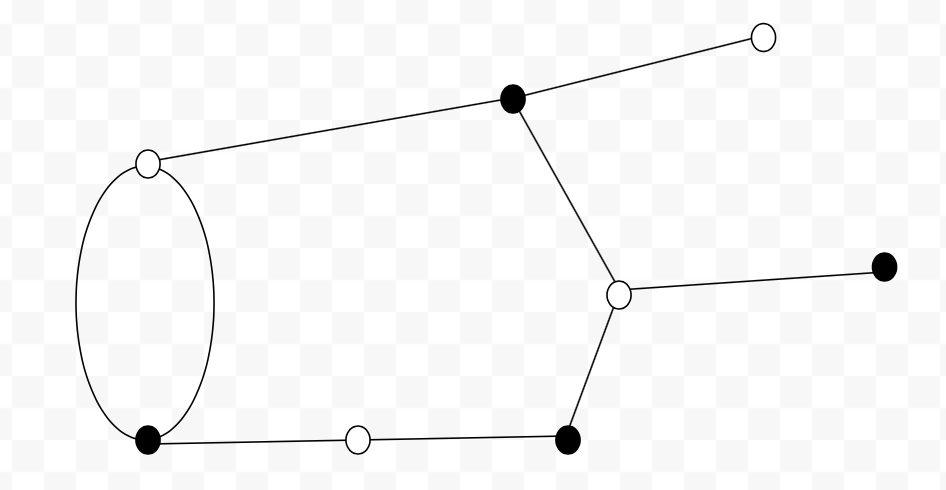
\includegraphics[scale=0.4]{images_talk/example_of_hypermap.png}
    \end{figure}
\end{frame}

\begin{frame}{Natural Questions about Dessins}
    \begin{enumerate}
        \item Why ramified at 3 points?
            % fractional linear transformations --> so technically, the 0,1,infty can be arbitrarily chosen
        \item Any reason for $\{0,1,\infty\}$ being chosen as the set of ramification points?
            % Not really. We could generalize our definition if we want as can map any 3 points to any other 3 points on Riemann sphere.
        \item Why compact? Why oriented?
            % compactness allows us to describe graphs on RS as algebraic curves (RECALL CORRESPONDENCE TO ALGEBRAIC CURVES)
            % oriented because how we will construct the dessins and associating positive/negative orientations (TO BE SHOWN)
        \item Why are Dessins defined this way?
        \item and most importantly, the point of all this?
            % jokeeeee
    \end{enumerate}
\end{frame}

% CHALK: BELYI PAIRS AND DESSIN'S
    % keywords: belyi functions, belyi pairs, meromorphic functions
\begin{frame}{Encoding Dessins by permutations}
    \textbf{Important:} Hypermaps admit an encoding by triples of permutations $(\sigma,\alpha,\phi)$.
    \begin{figure}
        \centering
        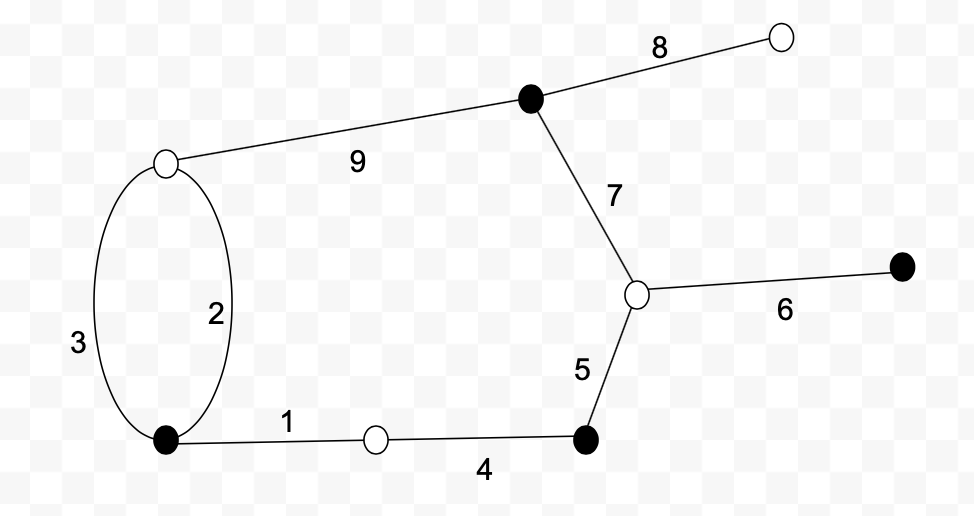
\includegraphics[scale=0.5]{images_talk/hypermap_permutations_encoding.png}
        \caption{\small{Hypermap labelling}}
    \end{figure}
\end{frame}

\begin{frame}{Encoding Dessins by permutations}
    \begin{figure}
        \centering
        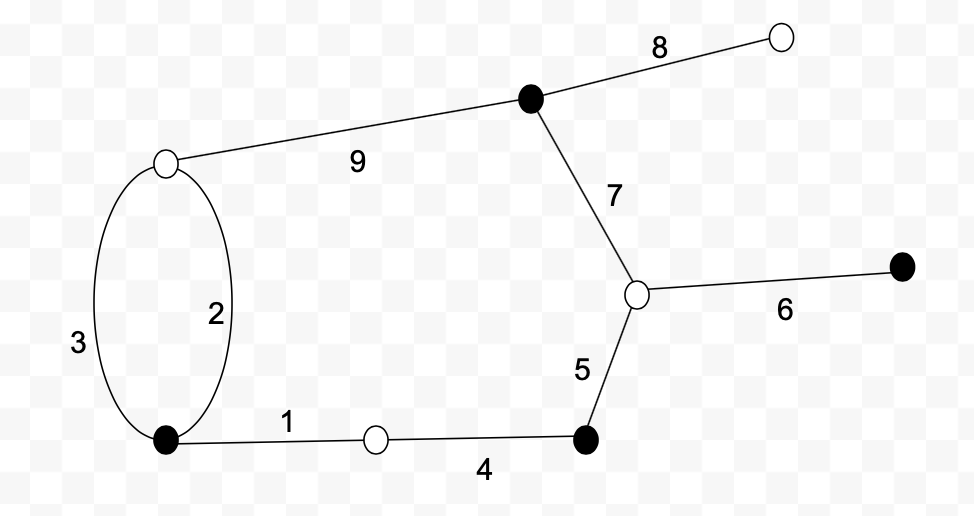
\includegraphics[scale=0.4]{images_talk/hypermap_permutations_encoding.png}
    \end{figure}
    
    \textbf{Important:} Ascribe a cycle to each vertex or face with the labelling in a \emph{counter-clockwise orientation}.
    
    \begin{align*}
        \sigma &= (123)(45)(6)(789)\\
        \alpha &= (293)(14)(567)(8)\\
        \phi &= (159)(2)(38764)\\
    \end{align*}
\end{frame}

% 4 MINS
% Note that not all vertices may be critical points even though pre-images of fibers
\begin{frame}{How do we create Dessins from Belyi pairs?}
    \begin{block}{Procedure}
    Let $(X,f)$ be a Belyi pair. 
    \begin{enumerate}
        \item $f^{-1}(0)$ = black vertices
        \item $f^{-1}(1)$ = white vertices
        \item Hypermap $H$ is the \emph{pre-image} of $[0,1]$ under $f$
        \item Degree of vertex $=$ \emph{multiplicity} of the pre-image of 0 or 1
        \item Each face corresponds to a pole (i.e. element of $f^{-1}(\infty)$) called a \emph{center}
        \item Degree of face $=$ \emph{multiplicity} of the pole
    \end{enumerate}
    \end{block}
    
    \begin{example}
    Imagine the following polynomial defined on the Riemann sphere $\hat{\CC}$.
    \begin{center}
    \large{
        $f(x) = -\frac{(x-9)(x-1)^3}{64x} = 1 - \frac{(x^2 - 6x - 3)^2}{64x} $
    }
    \end{center}
    \end{example}
\end{frame}

% 2 MINS
% NON-TRIVIAL Question being answered: Now, do you think we can create a Belyi pair from a Dessin? Can we identify the polynomial function and the Riemann surface from a combinatorial structure on a surface?

% can recreate RS that Dessin is defined on up to homeomorphism
\begin{frame}{Belyi function from a Dessin}
    \begin{figure}
        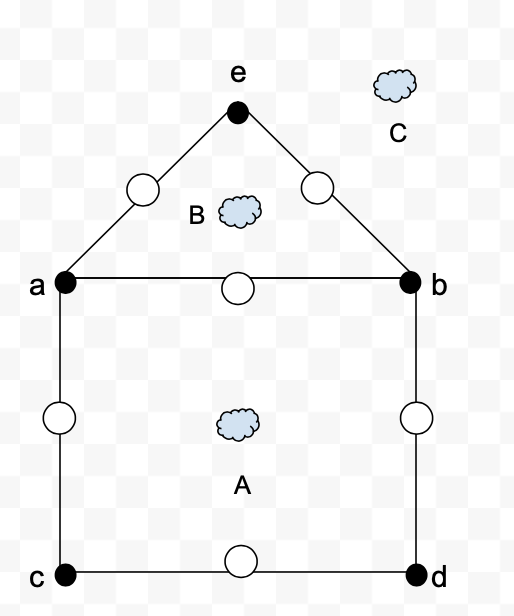
\includegraphics[scale=0.5]{images_talk/Belyi_from_dessin.png}
        \caption{\small{A harmless dessin}}
    \end{figure}
    \begin{align*}
        f(x) = K\frac{(x-a)^3(x-b)^3(x-c)^2(x-d)^2(x-e)^2}{(x-A)^4(x-B)^3(x-C)^5}
    \end{align*}
\end{frame}

\begin{frame}{Equations}
    \begin{align*}
        f(x) &= K\frac{(x^2 + px + q)^3(x^3 + rx^2 + sx + t)^2}{(x-A)^4(x-B)^3(x-C)^5}
    \end{align*}
    
    \begin{align*}
        f(x) - 1 &= K\frac{(x^6 + mx^5 + nx^4 + ux^3 + vx^2 + wx + z)^2}{(x-A)^4(x-B)^3(x-C)^5}
    \end{align*}
    
    Exactly 15 unknowns with 12 algebraic equations! Oh no!
\end{frame}

\begin{frame}{Equations}
    \begin{align*}
        f(x) &= K\frac{(x^2 + px + q)^3(x^3 + rx^2 + sx + t)^2}{(x-A)^4(x-B)^3(x-C)^3}
    \end{align*}
    
    \begin{align*}
        f(x) - 1 &= K\frac{(x^6 + mx^5 + nx^4 + ux^3 + vx^2 + wx + z)^2}{(x-A)^4(x-B)^3(x-C)^3}
    \end{align*}
    
    Exactly 15 unknowns with 12 algebraic equations! or oh yes?
\end{frame}

% 2 to 3 MINS
\begin{frame}{The Good Stuff}
    \begin{theorem}[Belyi's Theorem]
        Let $X$ be a compact Riemann surface. 
        
        $X$ admits a model over the field of algebraic numbers $\Bar{\QQ}$ if and only if there exists a meromorphic $f : X \to \hat{\CC}$ such that $(X,f)$ is a Belyi pair.
    \end{theorem}
\end{frame}

% 0.5 MIN
% Quote by Grothendieck on significance of Belyi's theorem
\begin{frame}{Starstruck}
\begin{exampleblock}{}
    This discovery, which is technically so simple, made a very strong impression on me, and it represents a {\color{blue} decisive turning point in the course of my reflections}, a shift in particular of my centre of interest in mathematics, which suddenly found itself strongly focussed. I do not believe that a {\color{blue} mathematical fact has ever struck me quite so strongly as this one, nor had a comparable psychological impact.} This is surely because of the very familiar, non-technical nature of the objects considered, of which any {\color{blue} child’s drawing} scrawled on a bit of paper (at least if the drawing is made without lifting the pencil) gives a perfectly explicit example.
  \vskip5mm
  \hspace*\fill{\small--- Alexander Grothendieck, \textit{Esquisse d'un Programme (1984)}}
\end{exampleblock}
\end{frame}

% 1 MIN
% Which RS corresponds to Dessins? Exactly those over the algebraic numbers. Relationship between combinatorics, complex analytic objects and algebraic curves.
\begin{frame}{Moment of Reflection}
    \begin{figure}
        \centering
        
\includegraphics[scale=0.3]{images_talk/moment_of_reflection.jpg}
    \end{figure}
\end{frame}

% 2 MINS
% keywords: fundamental theorem of Galois theory, faithful action, absolute Galois group of rationals

% begin with realizing the permutation on the coefficients then onto faithful action --> then to degree sequences as an invariant
\begin{frame}{Action of Absolute Galois Group, Gal$(\Bar{\QQ} / \QQ)$}
    \begin{definition}[Gal$(\Bar{\QQ} / \QQ)$]
        Field automorphisms of $\Bar{\QQ}$ such that for each $\psi$ automorphism, we have that $\psi(x) = q$, $\forall q \in \QQ$ i.e. fixes the \emph{base field} $\QQ$.
    \end{definition}

    \begin{definition}[Faithful group action]
        Let $G$ be a group and $X$ be a set. Then we say $G$ has a \emph{faithful action} on $X$ if for all $g \in G$ where $g \ne e_G$, $\exists x \in X$ s.t. $g \cdot x \ne x$.
    \end{definition}

    \begin{theorem}
        Gal$(\Bar{\QQ} / \QQ)$ has a \emph{faithful action} on the set of Dessins. 
    \end{theorem}

    \vfill
    \begin{block}{\tiny{Keywords}}
    \tiny{Gal$(\Bar{\QQ} / \QQ)$, faithful group action, field automorphisms, Fundamental theorem of Galois theory, number fields}
    \end{block}
    % finite orbits (cuz of degree invariant) --> finite stabilizers
\end{frame}

% 1 MIN
% Exploration of some intriguing connections between more or less classical topology and complex analysis to much more modern developments in algebraic and arithmetic geometry, which provide new ways to look at the Galois group of rationals

% We can see that by such a visibly simple object as a triple of permutations $(\sigma,\alpha,\phi)$ acting transitively and satisfying the condition $\sigma\alpha\phi = 1$, a great many interesting mathematical structures are explored 
\begin{frame}{Main areas of explorations of Dessins}
    \begin{enumerate}
        \item Given a dessin, find explicit equations for the $X$ and $f$ constituting a Belyi pair $(X,f)$ (for different genus)
        \item Find a list of topological, combinatorial, algebraic invariants of dessins in the same Gal$(\Bar{\QQ} / \QQ)$ orbit
        \item ... and probably questions we don't know yet that we want to look into!
    \end{enumerate}
\end{frame}



\end{document}